\documentclass[12pt, a4paper]{article}
\usepackage[english, russian]{babel}
\usepackage[T2A]{fontenc}
\usepackage[utf8]{inputenc}
\usepackage[left=3cm,right=1.5cm,top=2cm,bottom=2cm,bindingoffset=0mm]{geometry}
\usepackage{titlesec}
\usepackage{amsmath}
\usepackage{setspace}
\usepackage[pdftex]{graphicx}
\usepackage{dsfont}
\usepackage{comment}
\usepackage[unicode, pdftex]{hyperref}
\usepackage{fancyhdr}
\usepackage{colortbl}
\usepackage{indentfirst}

\graphicspath{{C:/Users/9/Desktop/market_mod}}
\setlength{\parindent}{1.25cm}
\linespread{1.5}


\begin{document}

\pagestyle{fancy}
\fancyhf{}
\renewcommand{\headrulewidth}{0pt}

\begin{center}
САНКТ-ПЕТЕРБУРГСКИЙ ГОСУДАРСТВЕННЫЙ УНИВЕРСИТЕТ\\
Направление: 01.03.02 Прикладная математика и информатика \\
ООП: Прикладная математика, фундаментальная информатика и программирование \\
Кафедра технологии программирования \\

\vspace*{2cm}
\large \textbf{ОТЧЕТ О НАУЧНО-ИССЛЕДОВАТЕЛЬСКОЙ РАБОТЕ}
\end{center}
\vspace*{1.5cm}

\begin{flushleft}
\textbf{Тема задания:}
\end{flushleft}
\hspace{1cm} Исследование вероятностной модели предсказания лучшей цены в биржевом \\ стакане по трейдовым данным
\vspace*{0.5cm}

\begin{flushleft}
\textbf{Выполнил:}
\end{flushleft}
\hspace{1cm} Смирнов Алексей Артёмович, группа 21.Б02-пу 
\vspace*{0.5cm}

\begin{flushleft}
\textbf{Руководитель научно--исследовательской работы:}
\end{flushleft}
\hspace{1cm} Блеканов Иван Станиславович, кандидат технических наук, доцент, \\ заведующий кафедрой технологии программирования
 
 
\vspace*{7cm}
\begin{center}
САНКТ-ПЕТЕРБУРГ \\
2024
\end{center}

\newpage

\renewcommand{\contentsname}{\begin{center}Содержание\end{center}}
\tableofcontents

\newpage

\fancyfoot[C]{\thepage}

\section{Введение}

Одна из основных проблем любого участника рынка --- неполная информация о состоянии самого рынка. Соответственно, любой участник рынка желает получить как можно больше информации, на основе которой и будет принимать дальнейшие действия, так как чем большим объемом информации он владеет, тем более правильным будет само действие с точки зрения желаемых результатов. Для увеличения количества информации о рынке используют модели, которые основаны на том, что рынок есть сильно взаимосвязная система, поэтому, имея некоторую часть информации о состоянии системы, можно делать предположения о состоянии неизвестных частей системы по определенным законам, которые могут быть как строго математическими, так и эмпирическими.

Данная работа посвящена изучению одной вероятностной модели о биржевом стакане (Orderbook), где под термином биржевого стакана подразумевается некоторая рыночная структура, на которой взаимодействуют через посредника в виде биржи две стороны --- покупатели и продавцы. Более подробное описание биржевого стакана будет дано в разделе [000].

\subsection{Актуальность работы}
Изучаемая модель направлена на оценивание неизвестных, в определенный момент времени, параметров рынка, которые могут быть использованы для решения известной задачи Execution, которая является частью отрасли Financial Technologies, связанной с улучшением и оптимизацией финансовых услуг. Более формальное описание и обсуждение задачи Execution будет дано в разделе [000].

\subsection{Цели и задачи работы}
Основная цель работы --- оценить применимость предложенной модели, описать ситуации, при которых модель себя показывает лучше или хуже предполагаемого и, соответственно, определить практическую ценность данного статистического подхода.

\newpage

\section{Микроструктура биржевого стакана}

Биржа или биржевой стакан представляет собой две стороны рынка --- продавцов (ask сторона) и покупателей (bid сторона). Каждая сторона состоит из множества ценовых уровней (price levels), где каждый ценовой уровень является очередью предлагаемых объемов (на ask стороне предлагаемый объем на продажу, на bid стороне желаемый объем покупки), порядок очереди определяется порядком появления предложения на бирже. Соответственно, лучшая цена на ask стороне называется лучшей ценой продажи, а лучшая цена на bid стороне, аналогично, называется лучшей ценой покупки.

\hypertarget{Orderbook}{
\begin{figure}[htbp]
\center{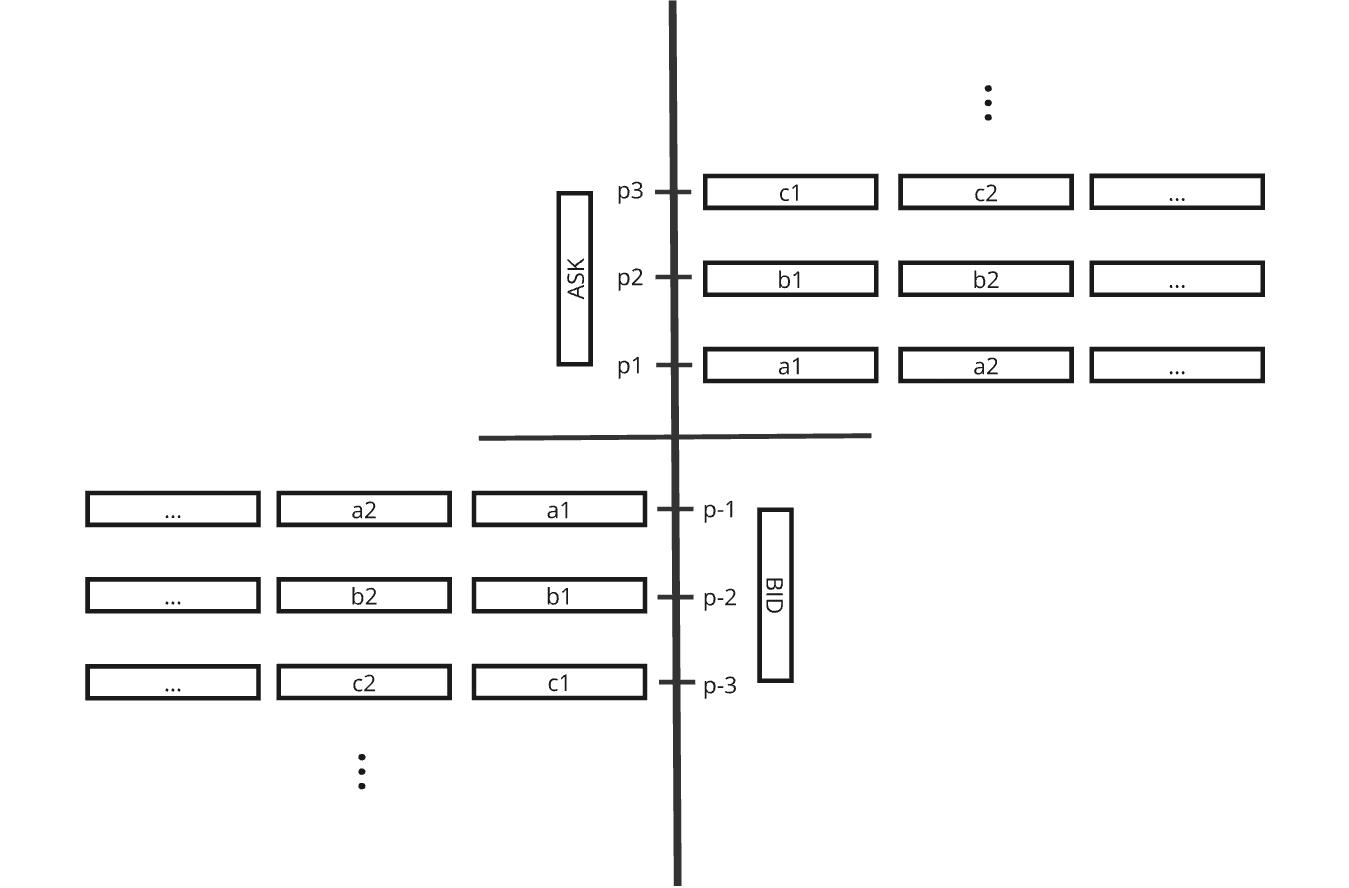
\includegraphics[width=1\textwidth]{Orderbook.png} Рисунок 1 --- Микроструктура биржевого стакана}
\end{figure}}

Как показано на $\hyperlink{Orderbook}{\text{Рисунке 1}}$, значения $p_i$ --- ценовые уровни, которые разбиты 
по объемам отдельных участников рынка, соответственно, общий объем, продающийся на конкретном уровне, есть сумма всех объемов в очереди.

\subsection{Основные характеристики биржевого стакана}

Величина $p_1 - p_{-1}$ есть величина спреда (spread), численно равный разности лучшей цены ask стороны и лучшей цены bid стороны, но имеющий прямое отношение к волатильности продукта, а именно, чем он больше, тем менее волатилен продукт. Это объясняется тем, что современная рыночная теория предполагает, что в каждый конкретный момент продукт имеет эталонную цену $(p_{ref})$, то есть истинную цену продукта в данный момент времени, купив или продав продукт по этой цене участник рынка считает, что он ничего не потерял и ничего не приобрел, следовательно желание продавцов --- продать продукт по большей цене, чем та, которую они считают для себя $p_{ref}$, а желание покупателей --- купить продукт дешевле, чем их субъективное представление о значении $p_{ref}$. Получаем, что значение $p_{ref}$ должно лежать в промежутке между лучшими ценами в стабильном состоянии биржевого стакана, так как иначе будет существовать такой ценовой уровень, по которому участники рынка будут считать выгодным для себя заключить сделку и, следовательно, этот ценовой уровень исчезнет. Очевидно, что ни один участник рынка точно не может знать значение $p_{ref}$, но каждый знает, что это значение находится внутри спреда и каждый участник рынка имеет ожидания по его движению в сторону увеличения или уменьшения, поэтому, если продукт является высоковолатильным, то частота сделок позволяет всем участникам рынка уточнить значение $p_{ref}$ и иметь более точные представления о его движении на коротких промежутках времени. Это означает, что интервал возможных значений $p_{ref}$ уменьшается для всех участников рынка, из-за чего ценовые уровни могут существовать довольно близко к истинному значению $p_{ref}$, так как не находится достаточное количество участников рынка, для которых данный уровень принадлежит их ожидаемому интервалу возможных значений $p_{ref}$. Иными словами, спред есть ожидаемый интервал возможных значений $p_{ref}$, согласованный всеми участниками рынка и ,как было показано выше, для высоковолатильных продуктов характерно иметь меньшую величину спреда, чем для низковолатильных, у которых участники рынка имеют меньше информации о значении $p_{ref}$ и, соответственно, ожидаемый интервал возможных значений $p_{ref}$ больше, то есть величина спреда больше.

Также стоит упомянуть, что на практике все численные значения на бирже принимают дискретные значения и величина между соседними значениями есть тик (tick). Например, для вычисления среднего значения цены продукта $(p_{mid})$, которую часто использую для оценки $p_{ref}$, применяют следующую формулу $\hyperlink{qrm}{[1]}$:

\[
\left\{
\begin{array}{cc}
\displaystyle \frac{p_1 + p_{-1}}{2} \quad \quad & if \quad \displaystyle\frac{p_1 + p_{-1}}{2} \notin \mathds{Z} \cdot t, \\
\displaystyle \frac{p_1 + p_{-1}}{2} \pm \frac{t}{2} \quad \quad & if \quad\displaystyle \frac{p_1 + p_{-1}}{2} \in \mathds{Z} \cdot t
\end{array}\right.,
\eqno(1)
\hypertarget{1}
\]
где $t$ - величина тика ценовых уровней. Суть формулы $\hyperlink{1}{(1)}$ в том, что значение $p_{ref}$ должно быть недостижимым значением ценового уровня для участников рынка, так как в противном случае все сделки происходили бы на этом уровне.

\subsection{Взаимодействие участников рынка в биржевом стакане}
\subsection{Практические особенности работы с биржами}
\section{Модель}
\section{Практические результаты}








\begin{comment}
\hypertarget{qrm}
\end{comment}
\end{document}